\defChapterTarget{Database Design}
Di seguito vengono riportati gli schemi di design del database e della sua
struttura logica. Come è possibile notare, mancano sugli schemi le definizioni
di tre cardinalità diverse. Tuttavia è possibile ricongiungere le cardinalità
tra gli oggetti "Service" e "Event" a quelle già definite nel precedente
capitolo, lasciando solo quella tra "Event" e "Booking" da definire.\\
La cardinalità "Event"->"Booking" è da considerarsi pari al numero di
prenotazioni disponibili per ogni dato evento, il quale può variare dalle 20
alle 50 persone. Questo ovviamente tenendo in conto degli eventi alla quale è
possibile prenotarsi, esempi di eventi nella quale non vi è questo tipo di
necessità potrebbero essere le collette alimentari o le raccolte fondi.
    \section{Database Design}
    \begin{figure}[H] 
        \centering 
        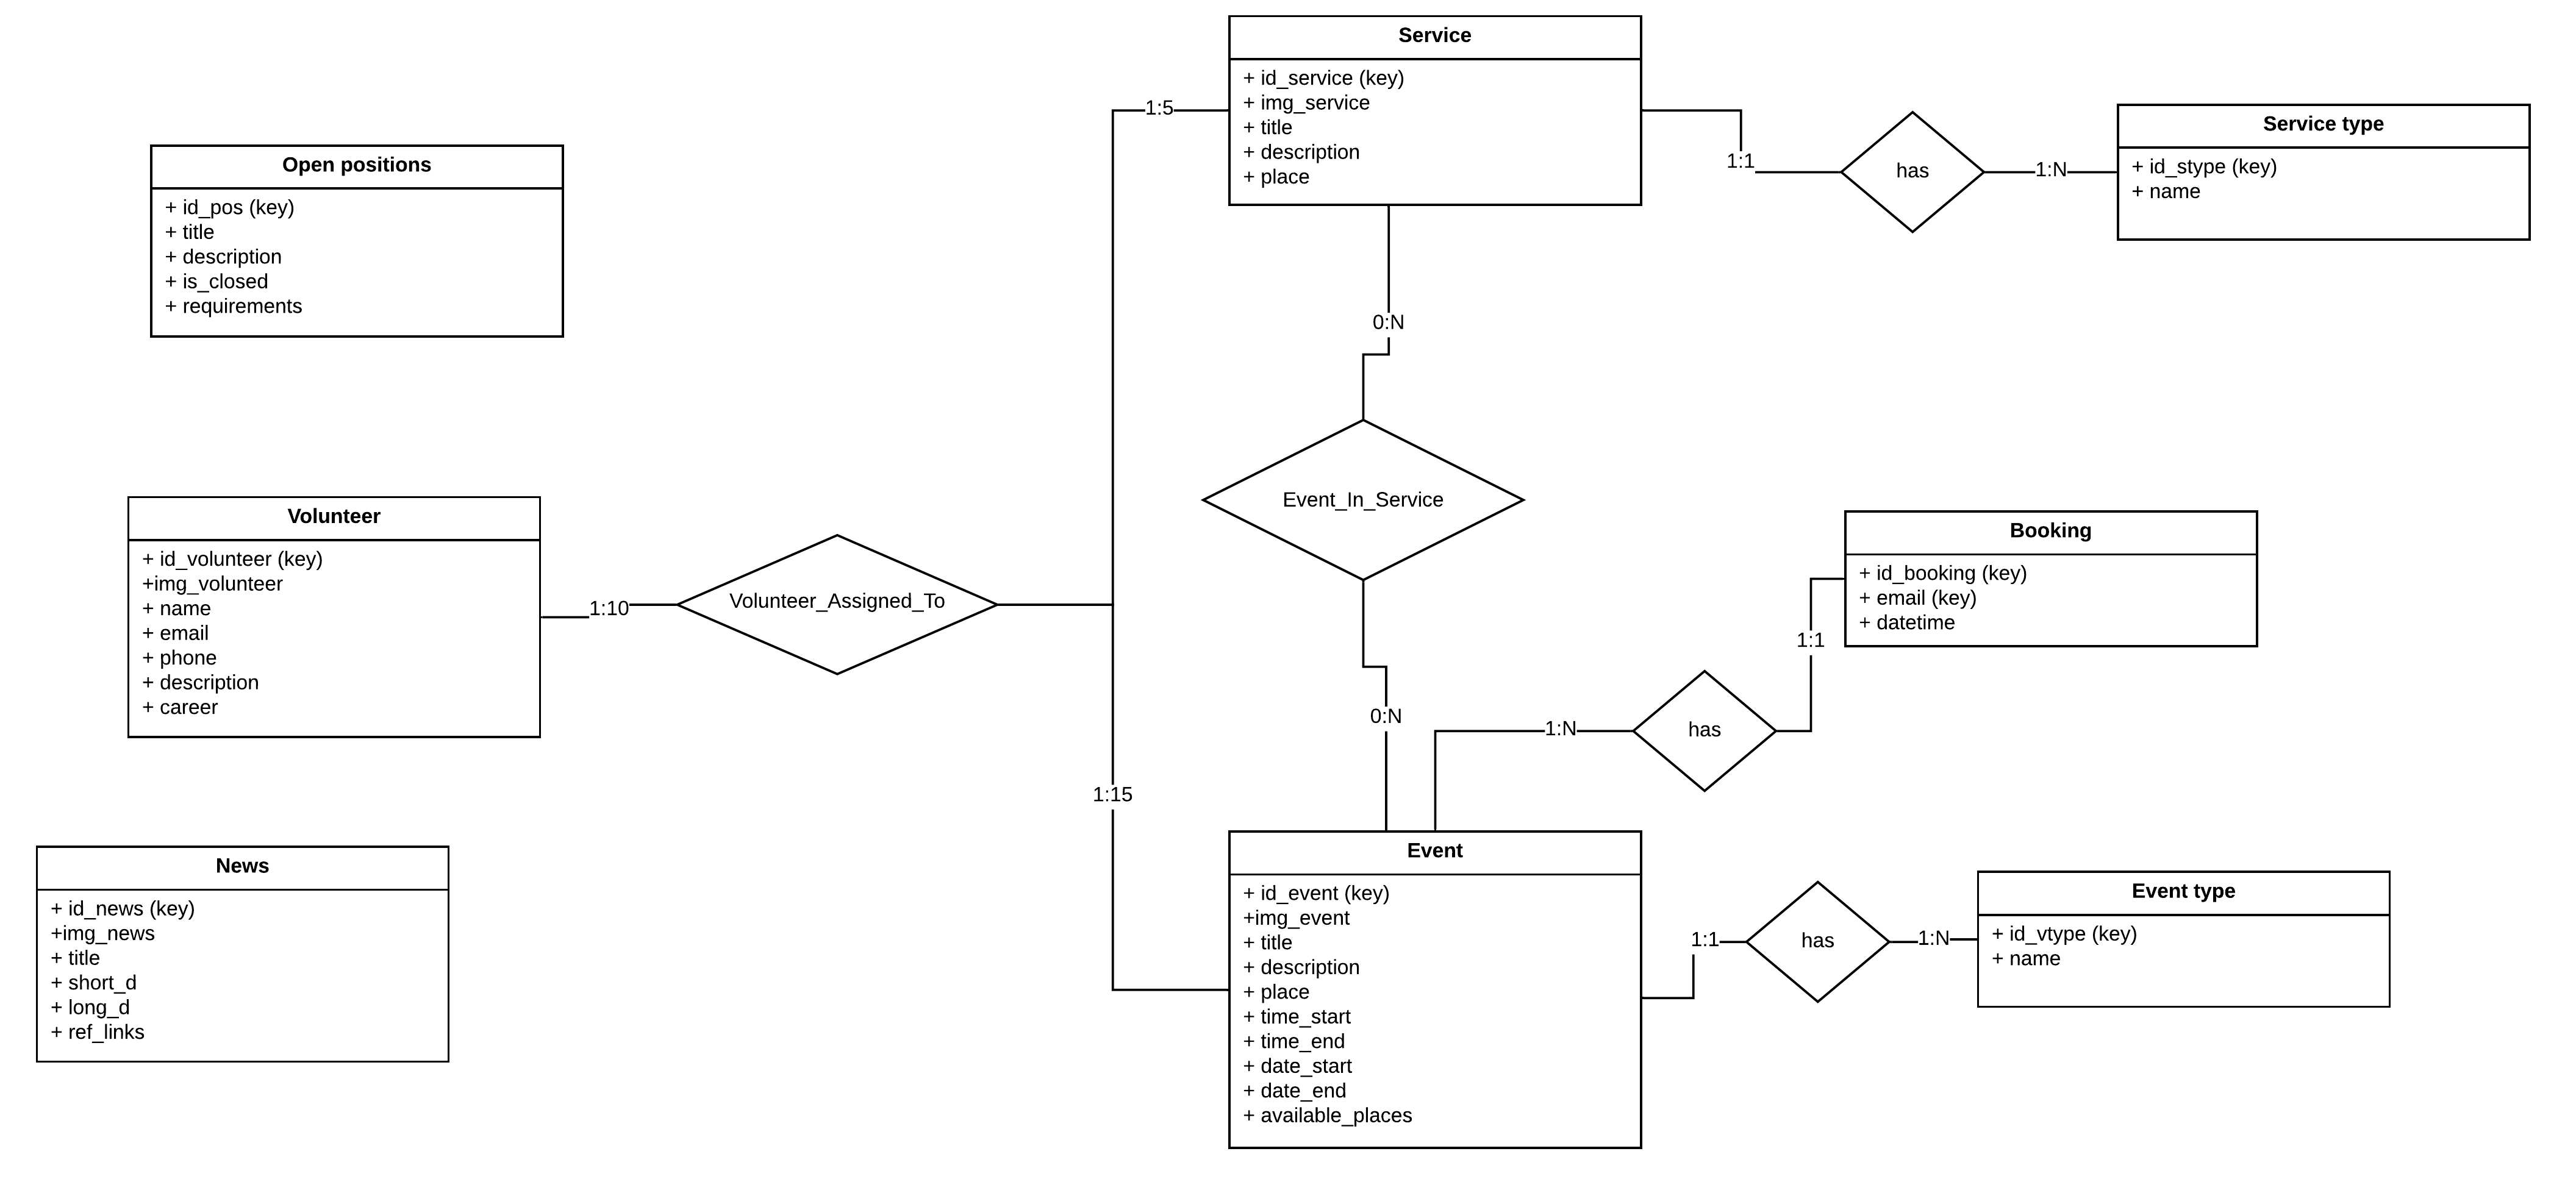
\includegraphics[scale=0.3]{resources/images/db.png}
    \end{figure}
    \section{Logical Design}
    \begin{figure}[H] 
        \centering
        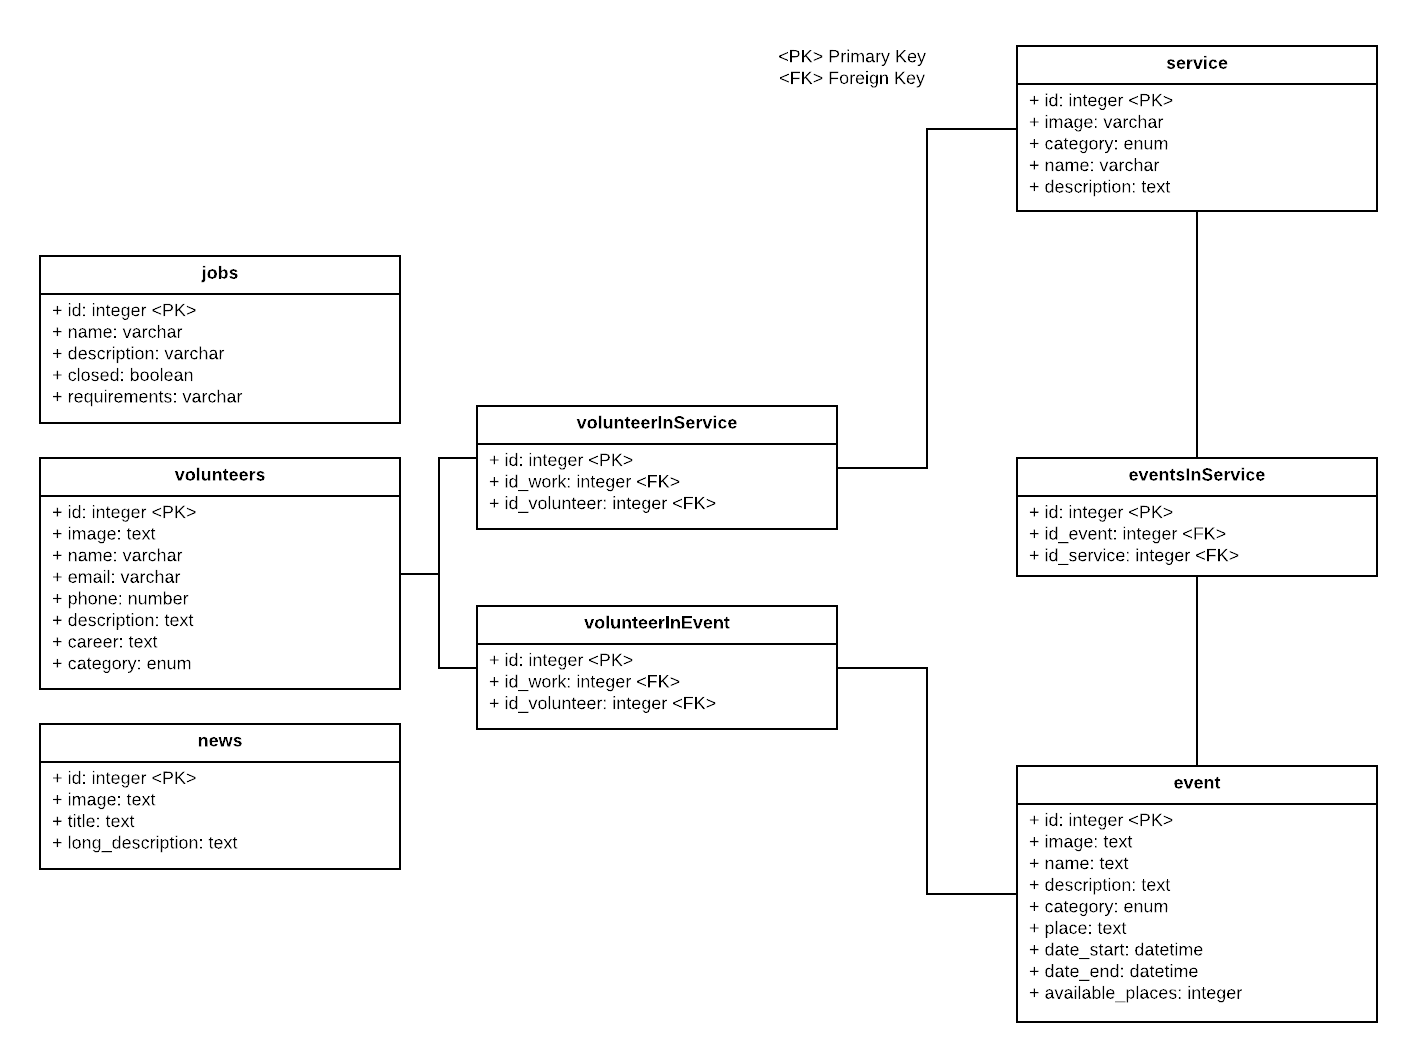
\includegraphics[scale=0.3]{resources/images/logical.png}
    \end{figure}